

\chapter*{3 System Design}
\label{intro}
\addcontentsline{toc}{chapter}{3 System Design}
\setcounter{chapter}{3}
\setcounter{section}{0}
\setcounter{figure}{0}
\setcounter{table}{0}
An autonomous system whereby C code and MCU configurations can be evaluated is needed as per \textbf{\ref{ps} \nameref{ps}}. It is standard practise for students, enrolled in the pertaining modules previously mentioned, to upload their projects as repositories (using for example GitHub). The scope of this project has been narrowed to focus on the STM32F4 family of \hyperref[listAbr]{MCU}s as per \textbf{\ref{scOfWrk} \nameref{scOfWrk}}. 
\\\\
The student repositories accessed, as part of this project, where provided by Dr Arno Barnard and are the repositories of students enrolled in E-Design 314 2020. The \hyperref[listAbr]{MCU} used, as part of this particular module in 2020, is the STM32F446RET. This implies that the \hyperref[listAbr]{MCU} was configured, programmed and debugged in STM32CubeIDE.

In order to evaluate \hyperref[listAbr]{MCU} configurations, student code must be assessed in an autonomous way. It would be nearly impossible (and very laborious) to manual assess all the student repositories in a particular year group:

\section{Autonomous System Outline}
\label{aso}


STM32CubeIDE has a very particular project structure consisting of various directories containing source code, included libraries, drivers and debugger files. These directories are contained within a project root directory and the general structure is highlighted below:

\begin{figure}[H]
\begin{center}
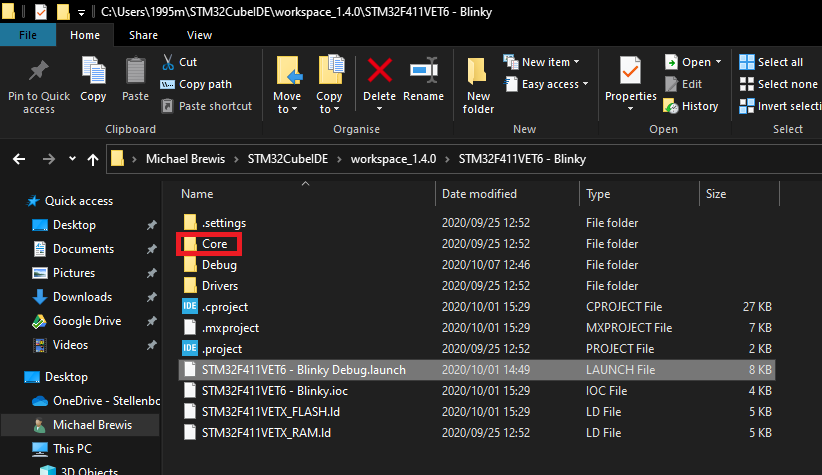
\includegraphics[width = 155mm]{stmProject.png}
\caption{STM32CubeIDE project structure}
\label{stmProj}
\end{center}
\end{figure}

Figure~\ref{stmProj} illustrates the default STM32CubeIDE project outline. It can be seen that any valid project contains a Core folder. This folder contains all the relevant C code and included libraries. It is this folder that is of relevance. The project illustrated above was created in STM32CubeIDE to blink an LED on an STM32F411 \hyperref[listAbr]{MCU}. It is, however, not part of the repositories sent by Dr Barnard. These repositories are, in fact, not depicted in order to maintain anonymity. 
\\\\
Anonymity is indeed a very important part of the automation process when it comes to evaluating student code. Once access to the repositories have been gained, it becomes necessary to remove any information from them that can be used to identify students. This will be elaborated upon in the sections to come.